\subsection{Sound and speed gauges}
The interview with the costumers (described in \cref{s2interview}) revealed that they use a gauge system to illustrate speeds and volume levels at the institution. 
The gauges used are pictured in \cref{gauges}.
Each gauge is from 0 to 10, and some of the levels have a pictogram associated.

\begin{figure}[h]
	\centering
        \begin{subfigure}[b]{0.5\textwidth}
                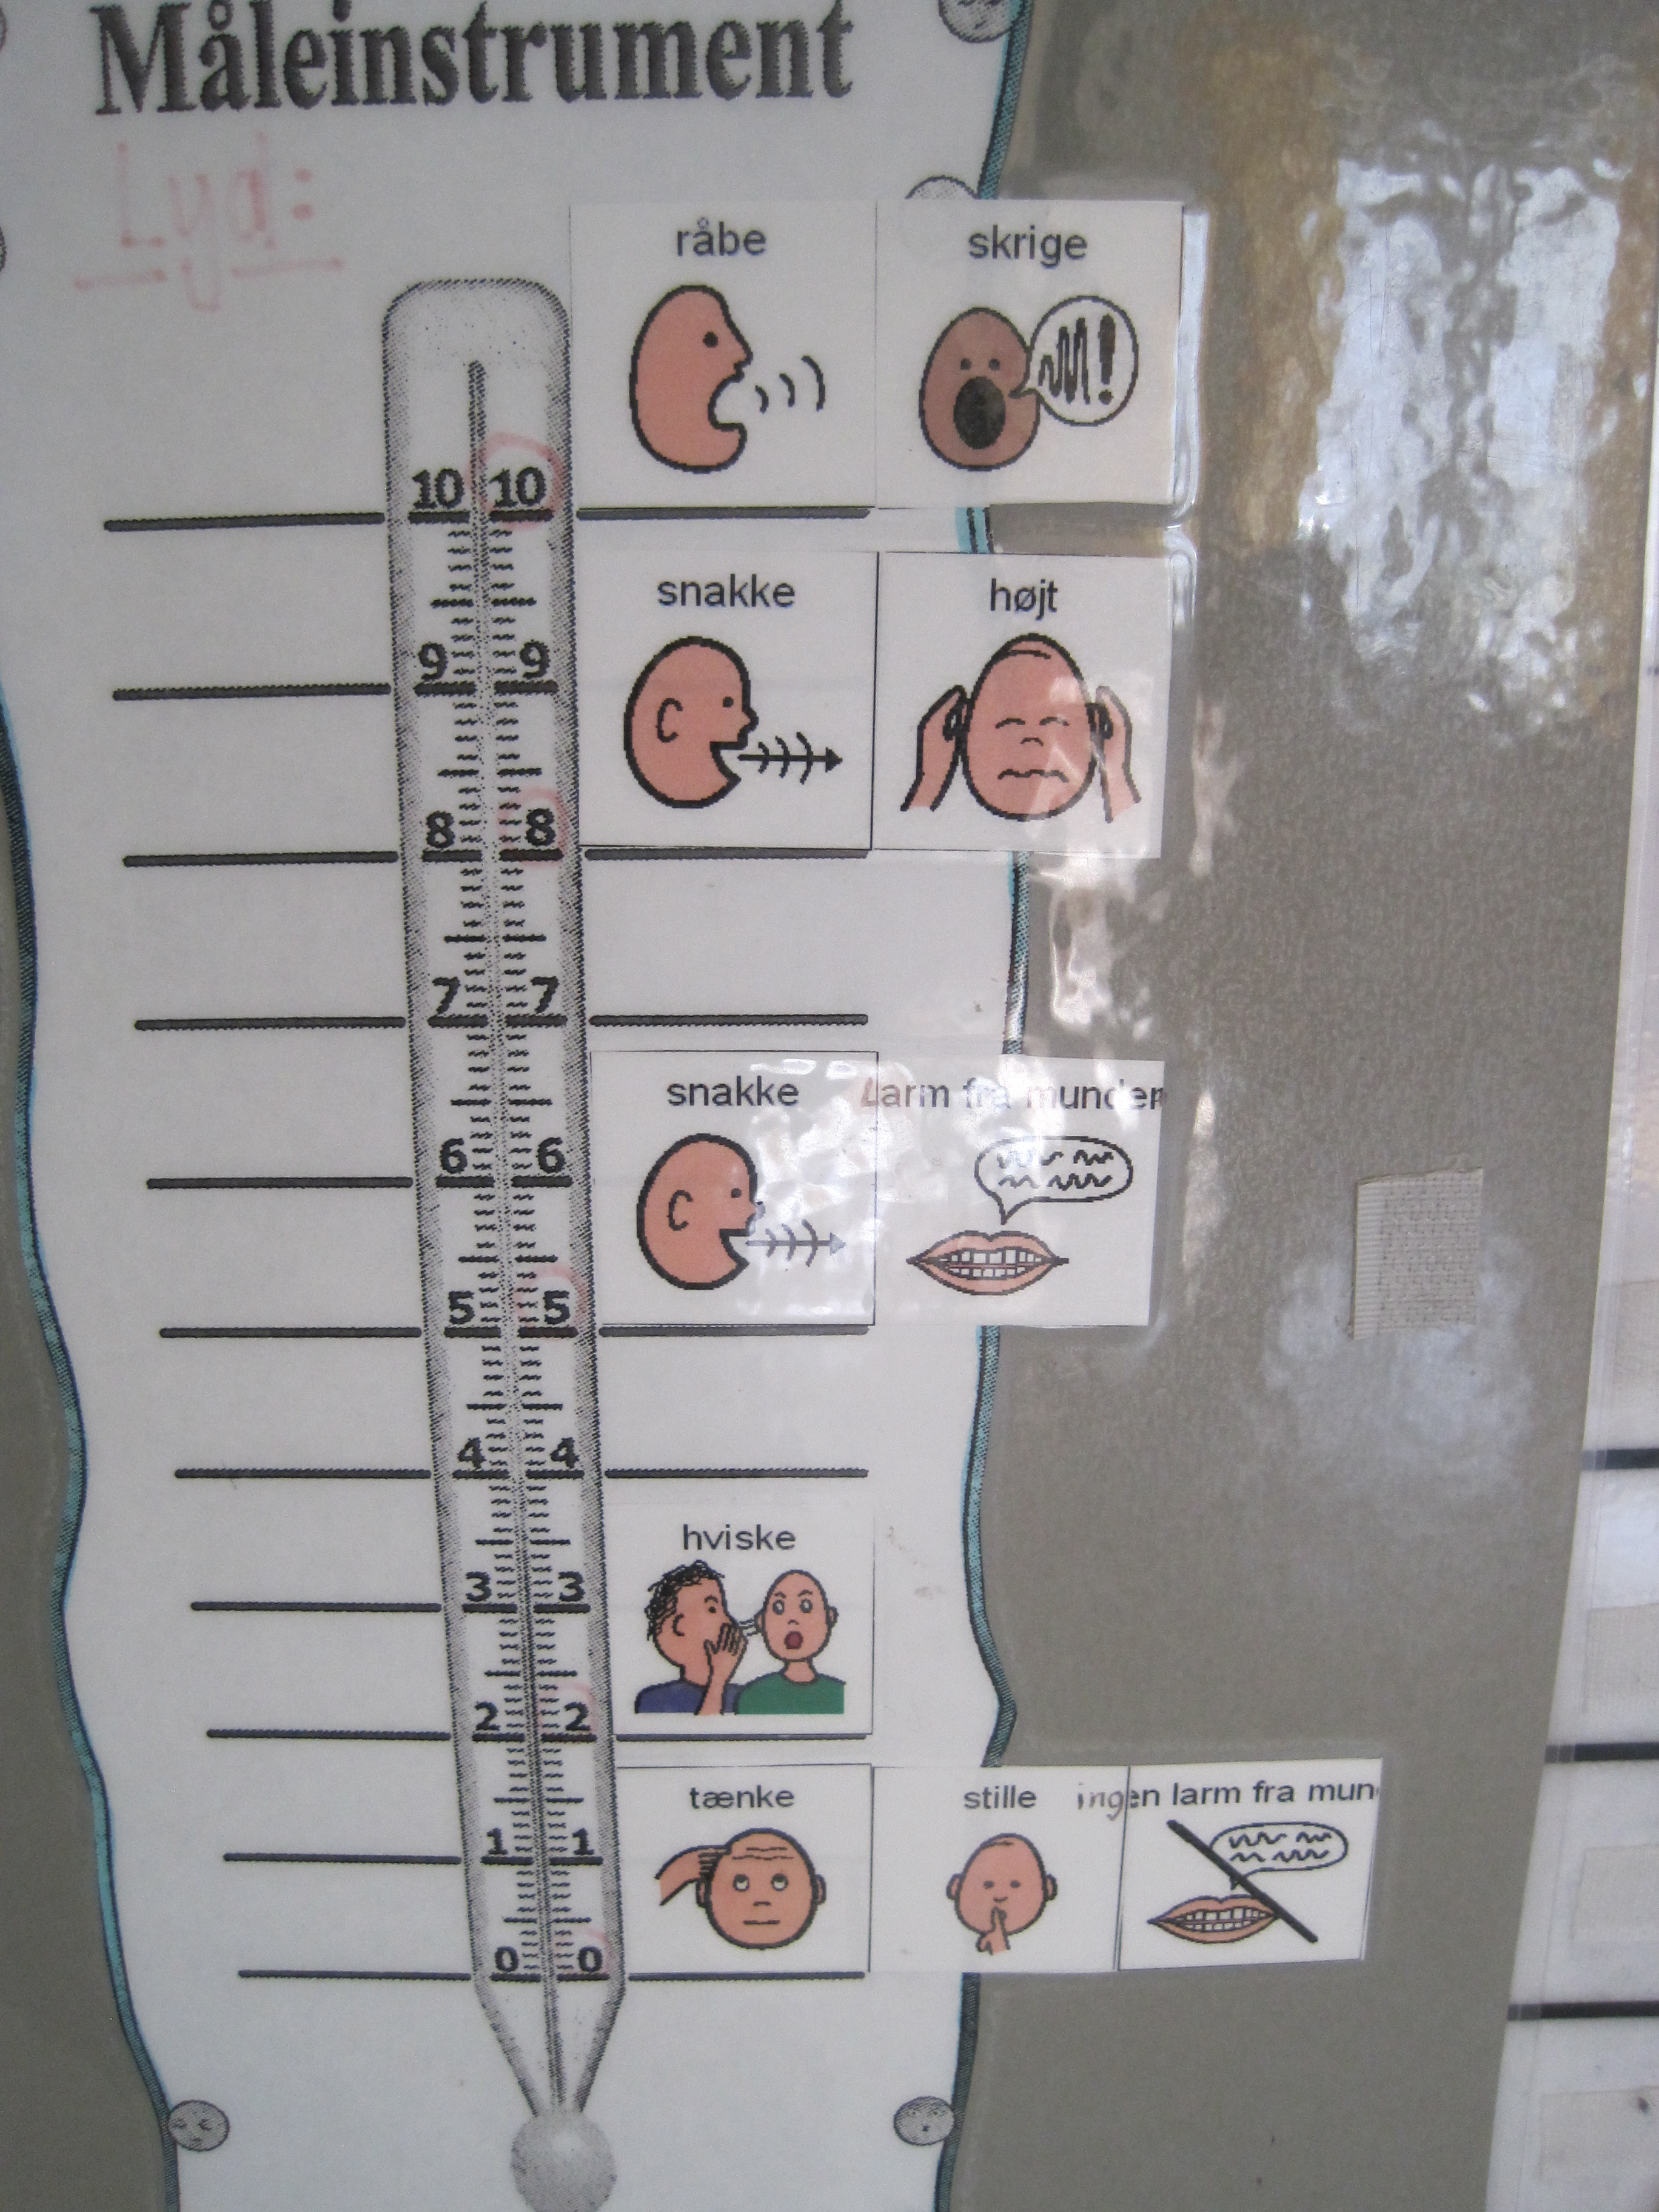
\includegraphics[width=\textwidth]{sound}
                \caption{The sound gauge}
                \label{soundgauge}
        \end{subfigure}%
        ~
        \begin{subfigure}[b]{0.5\textwidth}
                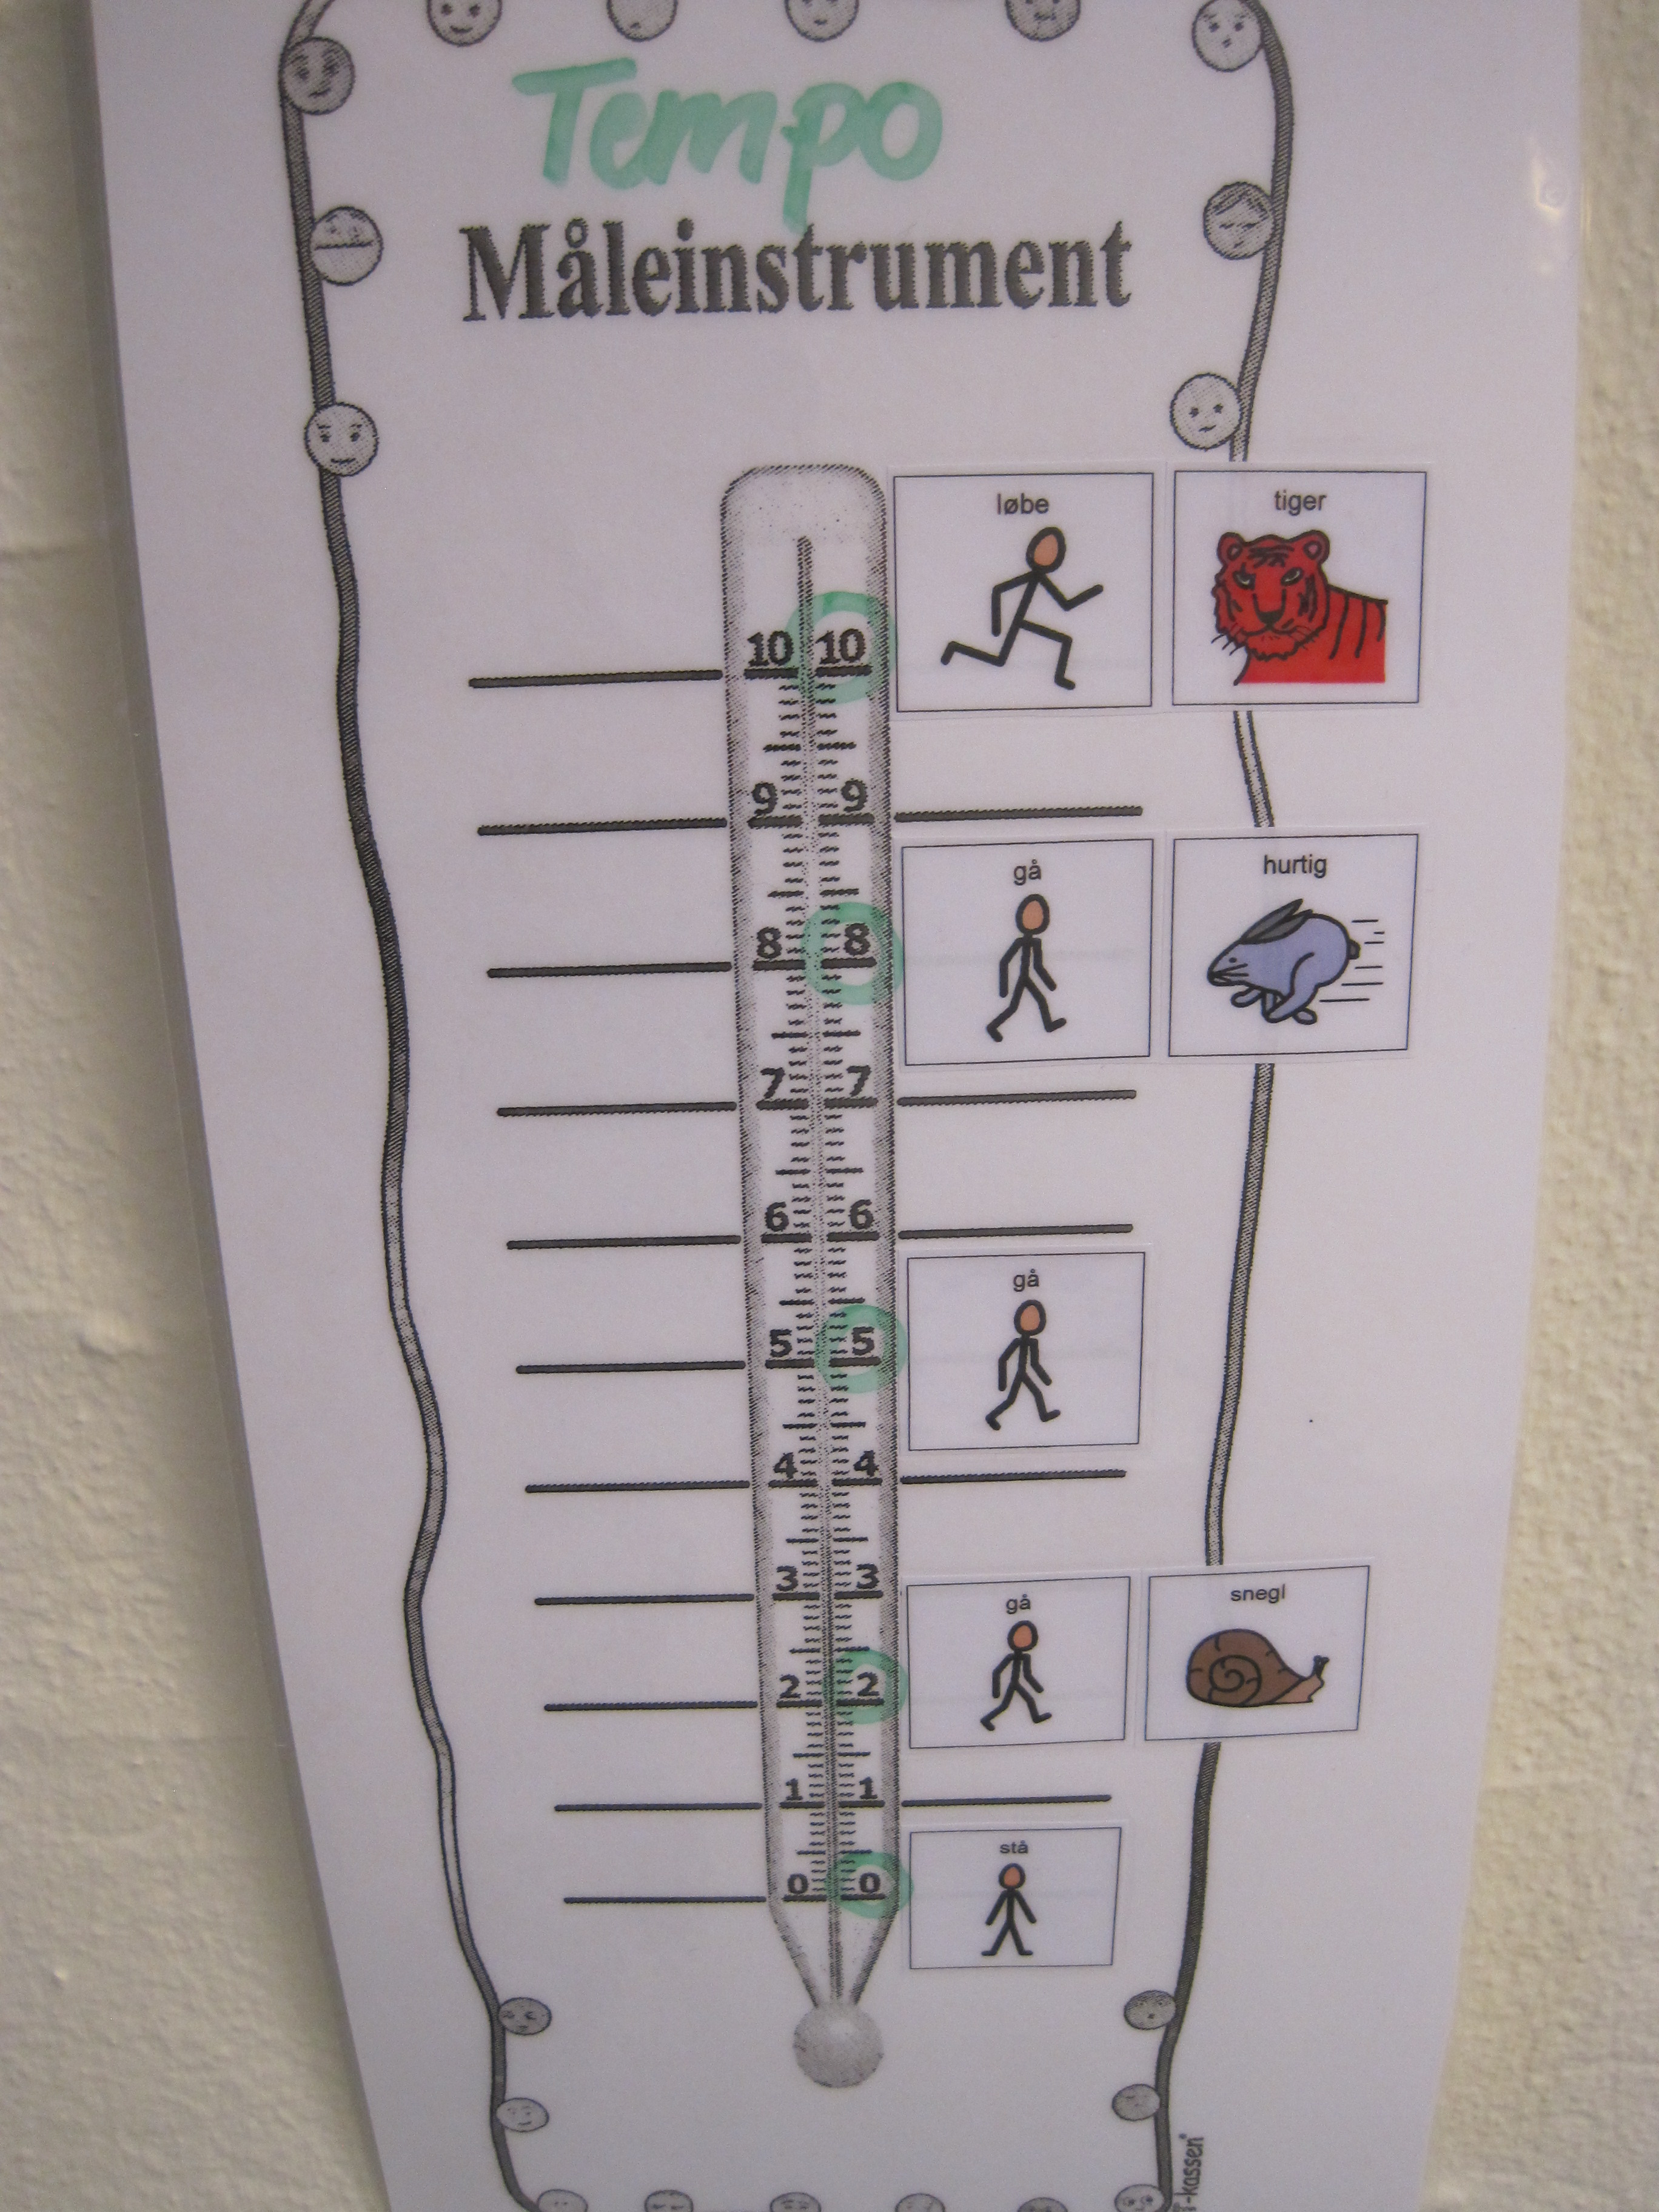
\includegraphics[width=\textwidth]{speed}
                \caption{The speed gauge}
                \label{speedgauge}
        \end{subfigure}
        \caption{The gauges used at 'Birken'}\label{fig:animals}
        \label{gauges}
\end{figure}

Several requirements (described in \cref{s2requirements}) is about incorporating these gauges in the game.
The requirements concerning the gauges are as follows:

\begin{enumerate}
\setcounter{enumi}{6}
\item \label{visualnumber} There is a digit between 0 and 10 displayed on the car as well as obstacles, representing the loudness level, based on its vertical position. 
\item \label{pictogram} Besides the scales from 0 to 10, both speed and loudness have pictograms illustrating some of the values on these scales.
\item \label{pause} It should be possible to pause the game. When the game is paused, a loudness-barometer is displayed next to the car, further visualizing the current loudness.
\item \label{speeditem} Speed is alterable. The speed level is represented as a digit between 0 and 10.
\end{enumerate}


\paragraph{Requirement \ref{visualnumber}} is met by drawing the number corresponding to the position of the object on the gauge. 
This can be seen on \cref{pausedstate}.

\paragraph{Requirement \ref{pictogram}} was not fulfilled in this sprint.


\paragraph{Requirement \ref{pause}} is partially fulfilled.
The pause functionality is achieved by having a pause button in the upper left corner. 
When the game is paused the game is faded out, and a representation of the gauge is placed left of the car so it is possible to see the full scale in the game area.
This can be seen on \cref{pause}.
This placeholder scale is to be replaced with a gauge similar to the one seen on \cref{soundgauge}.

The fulfilment of these two requirements can be seen on \cref{pausedstate}.

\begin{figure}
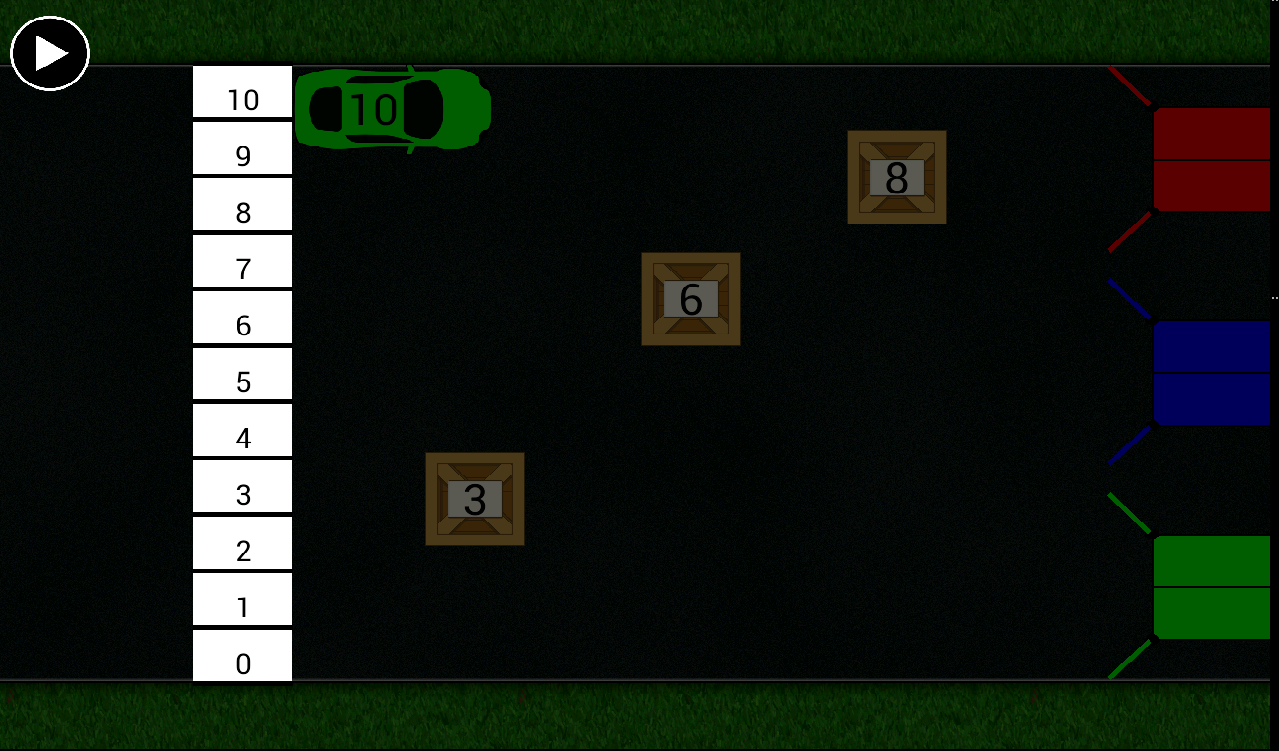
\includegraphics[width=\textwidth]{pause}	
\caption{The game in a paused state. The game is seen in the background and a sound gauge is shown left of the car}
\label{pausedstate}
\end{figure}


\paragraph{Requirement \ref{speeditem}} was only partially fulfilled in this sprint, by making the speed alterable. 
The gauges and pictograms are not yet visible on the settings module, which can be seen on \cref{speedsettings}.
The shown number is the value of speed used internally.
The speed is altered by pressing in the left or right side, decreasing or increasing the speed respectively.
These 'invisible' buttons are to be changed to pictograms from the gauge on \cref{speedgauge}.

\begin{figure}
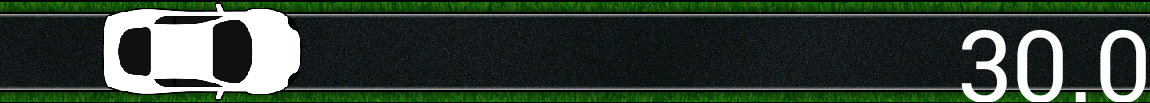
\includegraphics[width=\textwidth]{speedSettings}
\caption{The temporary implementation of alteration of the speed}
\label{speedsettings}
\end{figure}



